% TikZ pictures inside graphicx's transforms: \resizebox, \scalebox (one
% factor and two), \reflectbox, \rotatebox, and one transform inside another,
% in a display and inline. TeX draws each picture through the matrix around
% it; the pageless PDF, the browser's reference, must draw the captured
% picture with that matrix too. One page, so against_plain.
\documentclass{article}
\usepackage{tikz}
\usepackage{graphicx}
\pagestyle{empty}
\begin{document}
A paragraph before the pictures, long enough to break across lines
differently at every width the test tries, so that each picture below
moves when the text is reflowed.

\begin{center}
\resizebox{0.8\linewidth}{!}{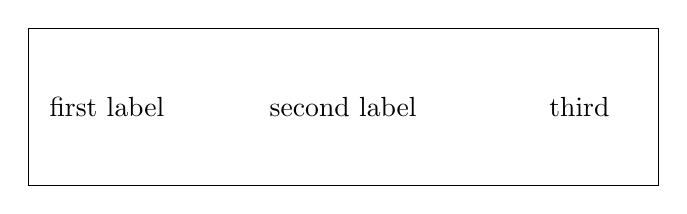
\begin{tikzpicture}
  \draw (0,0) rectangle (8,2);
  \node at (1,1) {first label}; \node at (4,1) {second label}; \node at (7,1) {third};
\end{tikzpicture}}
\end{center}
Inline: \scalebox{0.8}{\tikz\node[draw]{scaled node};},
\scalebox{1.2}[0.9]{\tikz\node{two factors};},
\reflectbox{\tikz\node{mirror};} and \rotatebox{90}{\tikz\node{turned};},
then some more text after them, so that the line breaks move them about.

\begin{center}
\scalebox{0.5}{\resizebox{6cm}{!}{\tikz{\draw (0,0) -- (3,1) node[right] {nested};}}}
\end{center}
Text after the last picture.
\end{document}
